\section{Container loading problems}

When the KP is generalized to multiple containers of varying volumes, it becomes a multi-container loading problem\footnote{When these dimensions are the same for all containers, the KP becomes a bin-packing problem.} (CLP). A model for solving such problems has been proposed by \textcite{CHEN1995}. The model concerns $m$ containers and $N$ items. To each item are assigned positioning variables $(x_i, y_i, z_i)$ and dimensions $(p_i, q_i, r_i)$ representing length, width and height, respectively. Much like \cref{eq:mip:3DKP Egeblad}, this model uses binary variables to represent the placement of item $i$ relative to item $k$: $a_{ik}$ (left), $b_{ik}$ (right), $c_{ik}$ (behind), $d_{ik}$ (front), $e_{ik}$ (below), $f_{ik}$ (above).

If item $i$ is assigned to container $j$, then $s_{ij} = 1$; otherwise, $s_{ij} = 0$. Rotations are introduced to the model through nine binary variables: $l_{xi}, l_{yi}, l_{zi}, w_{xi}, w_{yi}, w_{zi}, h_{xi}, h_{yi}, h_{zi}$. These variables determine which axis an item's length, width or height is parallel to. For example, if $l_{xi} = 1$, then item $i$ has its length parallel to the X axis.Evidently, the rotation variables must obey \cref{eq:clp rotation variable constraints}.

\begin{subequations}
    \label[constraint set]{eq:clp rotation variable constraints}
    \begin{align}
        &l_{xi} + l_{yi} + l_{zi} = 1,\\
        &w_{xi} + w_{yi} + w_{zi} = 1,\\
        &h_{xi} + h_{yi} + h_{zi} = 1,\\
        &l_{xi} + w_{xi} + h_{xi} = 1,\\
        &l_{yi} + w_{yi} + h_{yi} = 1,\\
        &l_{zi} + w_{zi} + h_{zi} = 1.
    \end{align}
\end{subequations}

From this set of equations, \textcite{CHEN1995} obtain the following equalities:

\begin{subequations}
    \label[equation set]{eq:clp rotation equation set}
    \begin{align}
        &l_{yi} = 1 - l_{xi} - l_{zi},\\
        &w_{xi} = l_{zi} - w_{yi} + h_{zi},\\
        &w_{zi} = 1 - l_{zi} - h_{zi},\\
        &h_{xi} = 1 - l_{xi} - l_{zi} + w_{yi} - h_{zi},\\
        &h_{yi} = l_{xi} + l_{zi} - w_{yi}.
    \end{align}
\end{subequations}

The model that \textcite{CHEN1995} propose is \cref{eq:ip:CLP Chen}. By replacing the rotation variables with the equations in \cref{eq:clp rotation equation set}, this model becomes simpler to solve.

\begin{subequations}
    \label{eq:ip:CLP Chen}
    \begin{align}
        \min &\sum_{j=1}^{m}L_jW_jH_jn_j - \sum_{i=1}^{N}p_iq_ir_i \label[expression]{eq:objective chen}\\
        \text{s. t.} &x_i + p_i l_{xi} + q_i w_{xi} + r_i h_{xi} \leq x_k + (1 - a_{ik}) M, \, \forall i, k, \, i < k, \label[constraints]{eq:comp chen 1}\\
        &x_k + p_k l_{xk} + q_k w_{xk} + r_k h_{xk} \leq x_i + (1 - b_{ik}) M, \, \forall i, k, \, i < k, \label[constraints]{eq:comp chen 2}\\
        &y_i + q_i w_{yi} + p_i l_{yi} + r_i h_{yi} \leq y_k + (1 - c_{ik}) M, \, \forall i, k, \, i < k, \label[constraints]{eq:comp chen 3}\\
        &y_k + q_k w_{yk} + p_k l_{yk} + r_k h_{yk} \leq y_i + (1 - d_{ik}) M, \, \forall i, k, \, i < k, \label[constraints]{eq:comp chen 4}\\
        &z_i + r_i h_{zi} + q_i w_{zi} + p_i l_{zi} \leq z_k + (1 - e_{ik}) M, \, \forall i, k, \, i < k, \label[constraints]{eq:comp chen 5}\\
        &z_k + r_k h_{zk} + q_k w_{zk} + p_k l_{zk} \leq z_i + (1 - f_{ik}) M, \, \forall i, k, \, i < k, \label[constraints]{eq:comp chen 6}\\
        &a_{ik} + b_{ik} + c_{ik} + d_{ik} + e_{ik} + f_{ik} \geq s_{ij} + s_{kj} - 1, \, \forall i, k, j, \, i < k \label[constraints]{eq:comp chen 7}\\
        &\sum_{j=1}^{m} s_{ij} = 1, \, \forall i, \label[constraints]{eq:all items in containers chen}\\
        &\sum_{i=1}^{N} s_{ij} \leq M n_j, \, \forall j, \label[constraints]{eq:items only in selected containers chen}\\
        &x_i + p_i l_{xi} + q_i w_{xi} + r_i h_{xi} \leq L_j + (1 - s_{ij}) M, \, \forall i, j, \label[constraints]{eq:items bound x chen}\\
        &y_i + q_i w_{yi} + p_i l_{yi} + r_i h_{yi} \leq W_j + (1 - s_{ij}) M, \, \forall i, j, \label[constraints]{eq:items bound y chen}\\
        &z_i + r_i h_{zi} + q_i w_{zi} + p_i l_{zi} \leq H_j + (1 - s_{ij}) M, \, \forall i, j, \label[constraints]{eq:items bound z chen}\\
        &l_{xi}, l_{yi}, l_{zi}, w_{xi}, w_{yi}, w_{zi}, h_{xi}, h_{yi}, h_{zi} \in \{0,1\}, \, \forall i\\
        &a_{ik}, b_{ik}, c_{ik}, d_{ik}, e_{ik}, f_{ik}, s_{ij}, n_j \in \{0,1\}, \, \forall i\\
        &x_i, y_i, z_i \geq 0.
    \end{align}
\end{subequations}

\cref{eq:objective chen} defines the CLP's objective to minimize the container volume that goes unused. Decision variables $n_j$ indicate whether a container has been selected or not. \cref{eq:comp chen 1,eq:comp chen 2,eq:comp chen 3,eq:comp chen 4,eq:comp chen 5,eq:comp chen 6} establish the relative placements of items in container $j$, in the same vein as \cref{eq:mip:3DKP Egeblad}. To guarantee that these alternative constraints work, \cref{eq:comp chen 7} force at least one of the positional variables to equal one, whenever two items share the same container.

\cref{eq:all items in containers chen} make it so every item is assigned to exactly one container. \cref{eq:items only in selected containers chen} ensure that items are only assigned to selected containers. Finally, \cref{eq:items bound x chen,eq:items bound y chen,eq:items bound z chen} make it impossible for items to breach their container's boundaries.

Our \href{https://github.com/phcentenaro7/IC-Knapsack/blob/7f581ff02334992a6181a06adbce668b528caeba/Knapsack/Chen/clp.jl#L27}{implementation} of this model and a \href{https://github.com/phcentenaro7/IC-Knapsack/blob/7f581ff02334992a6181a06adbce668b528caeba/Knapsack/Chen/clp.jl#L122}{visualization method} allows us to verify that this CLP model works when tested with the item set in \cref{tab:3DKP example items} and two $20\times20\times20$ containers. \cref{fig:clp example solution} shows the solution to this problem.

\begin{figure}[h]
    \centering
    \caption{Containers in an example solution to the CLP.}
    \label{fig:clp example solution}
    \begin{subfigure}{.4\textwidth}
        \centering
        \caption{Container 1}
        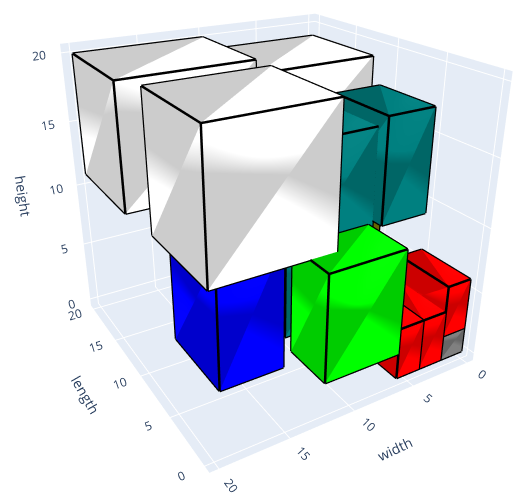
\includegraphics[width=\linewidth]{images/ChenExampleContainer1.png}
    \end{subfigure}
    \begin{subfigure}{.5\textwidth}
        \centering
        \caption{Container 2}
        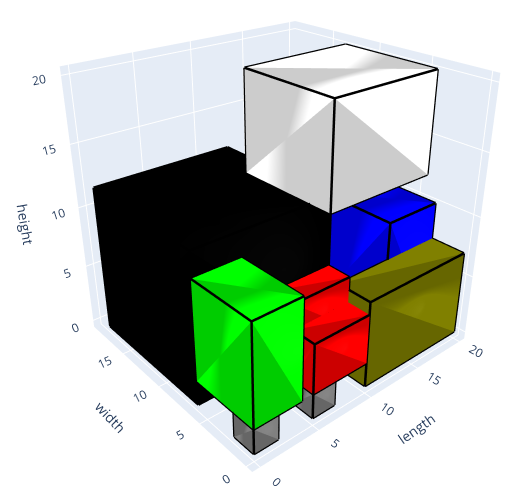
\includegraphics[width=0.8\linewidth]{images/ChenExampleContainer2.png}
    \end{subfigure}
\end{figure}